\subsection{任务三}

题目给出的PHILOX-2W算法是一种基于Feistel结构的分组密码，
其左右分支长度均为$W=8$bit，乘法常数为$M=0x9B$。
实验要求分析输入掩码分别为$(0,1)$、$(1,0)$、$(0,2)$、$(2,1)$
时的一轮线性掩码传播情况，并找出每组输入掩码对应的
输出偏差绝对值最大的前5个输出掩码及其偏差。

根据题目给出的轮函数，设输入状态为$(L,R)$，
轮密钥为$K$，一轮输出状态为$(L',R')$，则有
\[
L'=\operatorname{mullo}_W(R),
\]
\[
R'=\operatorname{mulhi}_W(R)\oplus L\oplus K,
\]
其中
\[
\operatorname{mulhi}_W(R)
=\left\lfloor\frac{R\cdot M}{2^W}\right\rfloor,
\qquad
\operatorname{mullo}_W(R)
=(R\cdot M)\bmod 2^W.
\]

设输入掩码为$\alpha=(\alpha_L,\alpha_R)$，
输出掩码为$\beta=(\beta_L,\beta_R)$，
则对应的线性近似式为
\[
\alpha_L\cdot L\oplus\alpha_R\cdot R
\oplus\beta_L\cdot L'\oplus\beta_R\cdot R'.
\]

将轮函数代入上述表达式，整理可得
\[
\begin{aligned}
&(\alpha_L\oplus\beta_R)\cdot L
\oplus\alpha_R\cdot R\oplus\beta_L\cdot\operatorname{mullo}_W(R)
\oplus\beta_R\cdot\operatorname{mulhi}_W(R)
\oplus\beta_R\cdot K.
\end{aligned}
\]

由于输入分支$L$在$\mathbf{F}_2^8$上均匀分布，
当$\alpha_L\neq\beta_R$时，
上述线性表达式关于$L$的取值均匀分布于0和1，
因此对应的线性偏差为0。
故只需考虑满足
\(
\beta_R=\alpha_L
\)
的输出掩码。

此时线性近似式化简为
\[
\alpha_R\cdot R
\oplus\beta_L\cdot\operatorname{mullo}_W(R)
\oplus\alpha_L\cdot\operatorname{mulhi}_W(R)
\oplus\alpha_L\cdot K.
\]

由于轮密钥$K$只影响线性近似式的常数项，
不会影响线性偏差的绝对值，因此实验中取$K=0$。

计算思路为：
先遍历题目给出的4组输入掩码
$\alpha=(\alpha_L,\alpha_R)$，
根据上述条件确定输出掩码右分支
$\beta_R=\alpha_L$，
再遍历全部$2^8$种输出左分支掩码$\beta_L$。
对于每组输入、输出掩码，遍历全部$2^8$种右分支输入$R$，
计算对应线性近似式是否为0。
统计其中为0的个数$N(\alpha,\beta)$，
并计算线性偏差
\[
\varepsilon(\alpha,\beta)
=\frac{N(\alpha,\beta)}{2^8}-\frac12.
\]

最后将所有输出掩码按照线性偏差的绝对值降序排列，
选取前5个输出掩码及其偏差。

记$\operatorname{par}(v)$为8比特数$v$中1的个数模2，
$\land$表示逐位与运算，
对应伪代码如算法~\ref{alg:task3-philox}所示。

\begin{algorithm}[H]
    \caption{PHILOX-2W一轮线性掩码传播分析}
    \label{alg:task3-philox}
    \begin{algorithmic}[1]
        \Require $W=8$，$M=0x9B$，
        输入掩码集合$\mathcal{A}=\{(0,1),(1,0),(0,2),(2,1)\}$
        \Ensure 各输入掩码对应的前5个输出掩码及其线性偏差

        \For{$(\alpha_L,\alpha_R)\in\mathcal{A}$}
            \State $T\gets\emptyset$
            \State $\beta_R\gets\alpha_L$

            \For{$\beta_L=0,\ldots,255$}
                \If{$(\beta_L,\beta_R)=(0,0)$}
                    \State \textbf{continue}
                \EndIf

                \State $N\gets 0$

                \For{$R=0,\ldots,255$}
                    \State $H\gets\left\lfloor R\cdot M/2^8\right\rfloor$
                    \State $D\gets(R\cdot M)\bmod 2^8$
                    \State $p\gets\operatorname{par}(\alpha_R\land R)$
                    \State $q\gets\operatorname{par}(\beta_L\land D)
                    \oplus\operatorname{par}(\beta_R\land H)$

                    \If{$p=q$}
                        \State $N\gets N+1$
                    \EndIf
                \EndFor

                \State $\varepsilon\gets N/256-1/2$
                \State $T\gets T\cup\{(\beta_L,\beta_R,\varepsilon)\}$
            \EndFor

            \State 按$|\varepsilon|$降序排列$T$
            \State $\mathrm{Result}[\alpha]\gets\operatorname{Top5}(T)$
        \EndFor

        \State \Return $\mathrm{Result}$
    \end{algorithmic}
\end{algorithm}

代码运行结果如图~\ref{fig:task3-philox}所示。

\begin{figure}[H]
    \centering
    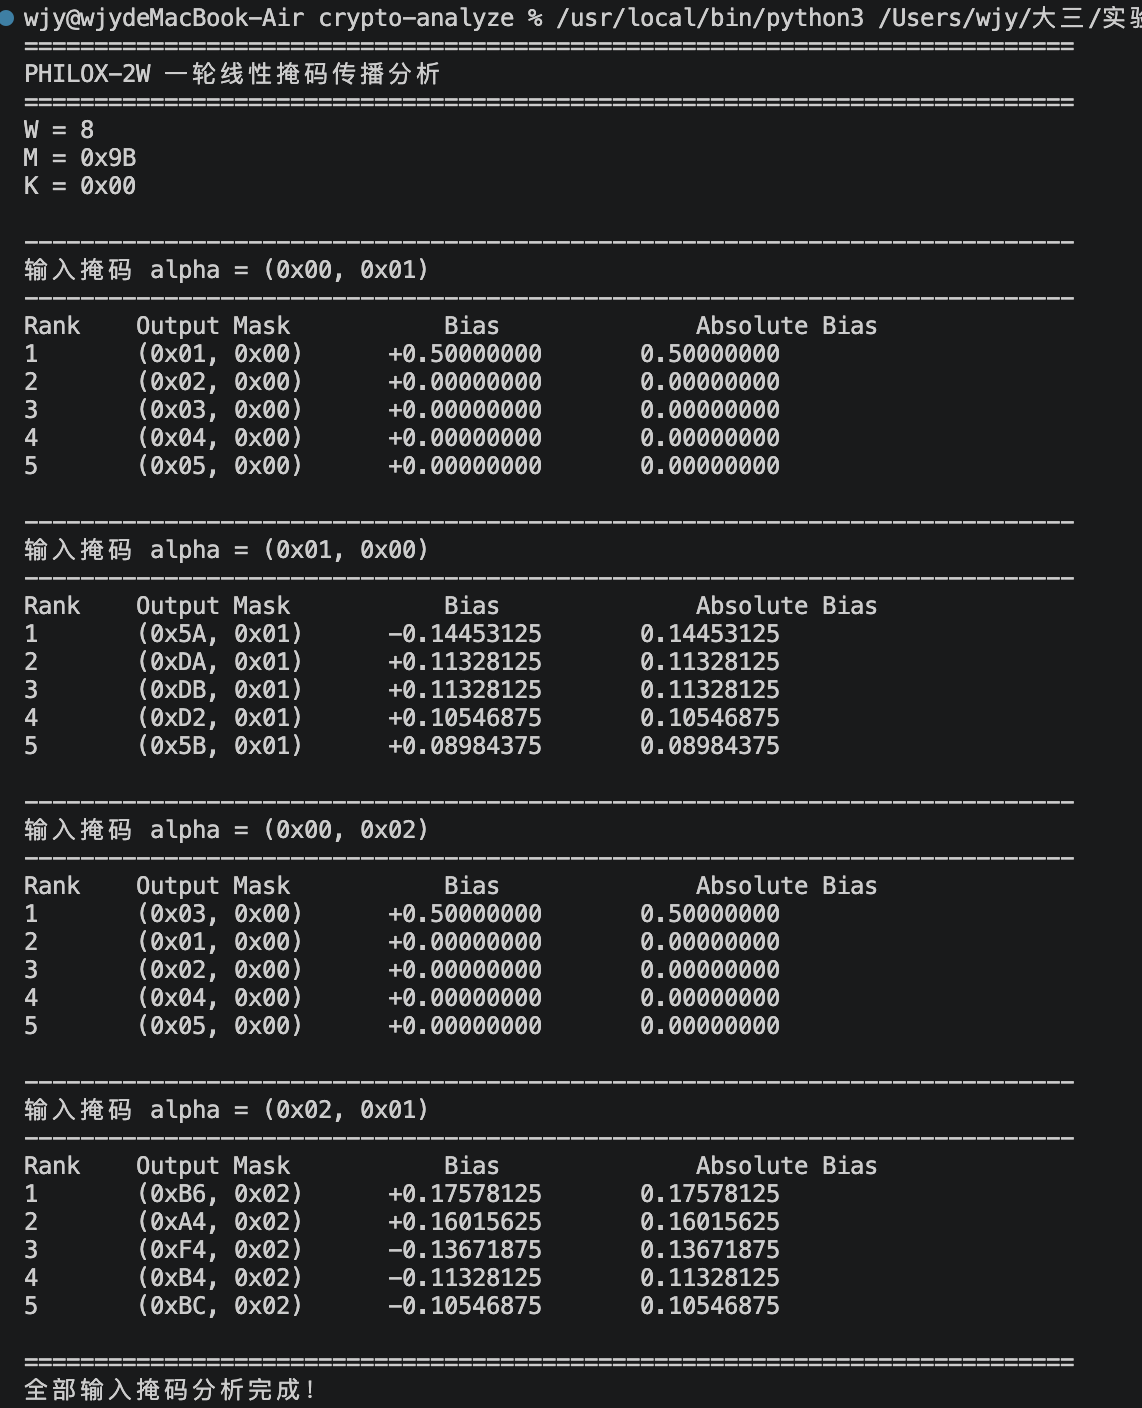
\includegraphics[width=\textwidth]{figures/task3.png}
    \caption{PHILOX-2W一轮线性掩码传播分析结果}
    \label{fig:task3-philox}
\end{figure}

由实验结果可知，4组输入掩码对应的最大绝对偏差分别为
$0.5$、$0.14453125$、$0.5$和$0.17578125$，
其对应的输出掩码分别为
$(0x01,0x00)$、$(0x5A,0x01)$、
$(0x03,0x00)$和$(0xB6,0x02)$。

其中，输入掩码$(0,1)$和$(0,2)$均存在绝对偏差为$0.5$
的输出掩码，说明对应线性关系以概率1成立。
而输入掩码$(1,0)$和$(2,1)$的最大绝对偏差均小于$0.5$，
表明对应的最佳线性近似存在一定的统计偏差，
但并非恒成立。

此外，利用PHILOX-2W轮函数的结构性质，
将输出掩码的搜索范围由$2^{16}$种缩小至$2^8$种，
并将每组掩码的计算由遍历$2^{16}$个输入状态
简化为遍历$2^8$个右分支输入，
在保证计算结果精确性的同时降低了计算复杂度。